\section*{CHAPTER 1. INTRODUCTION}
\addcontentsline{toc}{section}{\numberline{}CHAPTER 1. INTRODUCTION}

\setcounter{section}{1}
\setcounter{subsection}{0}
\setcounter{figure}{0}
\setcounter{table}{0}
\setcounter{equation}{0}

%============================================================%
\subsection{Background}

The rapid development of modern wireless communication systems has created
a growing demand for high data rate transmission, efficient spectrum
utilization, low latency, and reliable communication under challenging
channel conditions. Applications such as mobile broadband, video
streaming, Internet of Things (IoT), and fifth-generation (5G) wireless
networks require transmission techniques capable of operating efficiently
in multipath fading environments while maintaining acceptable complexity
and power consumption.

In wireless channels, transmitted signals often experience reflection,
diffraction, and scattering due to surrounding objects such as buildings,
vehicles, and terrain. As a result, multiple delayed copies of the signal
arrive at the receiver simultaneously, producing a phenomenon known as
multipath fading. This effect causes inter-symbol interference (ISI),
which significantly degrades communication performance.

\begin{equation}
\label{eq:received_signal}
r(t)=s(t)*h(t)+n(t)
\end{equation}

where $s(t)$ is the transmitted signal, $h(t)$ is the wireless channel
impulse response, and $n(t)$ represents additive noise.

\vspace{0.3cm}

\begin{figure}[H]
    \centering
    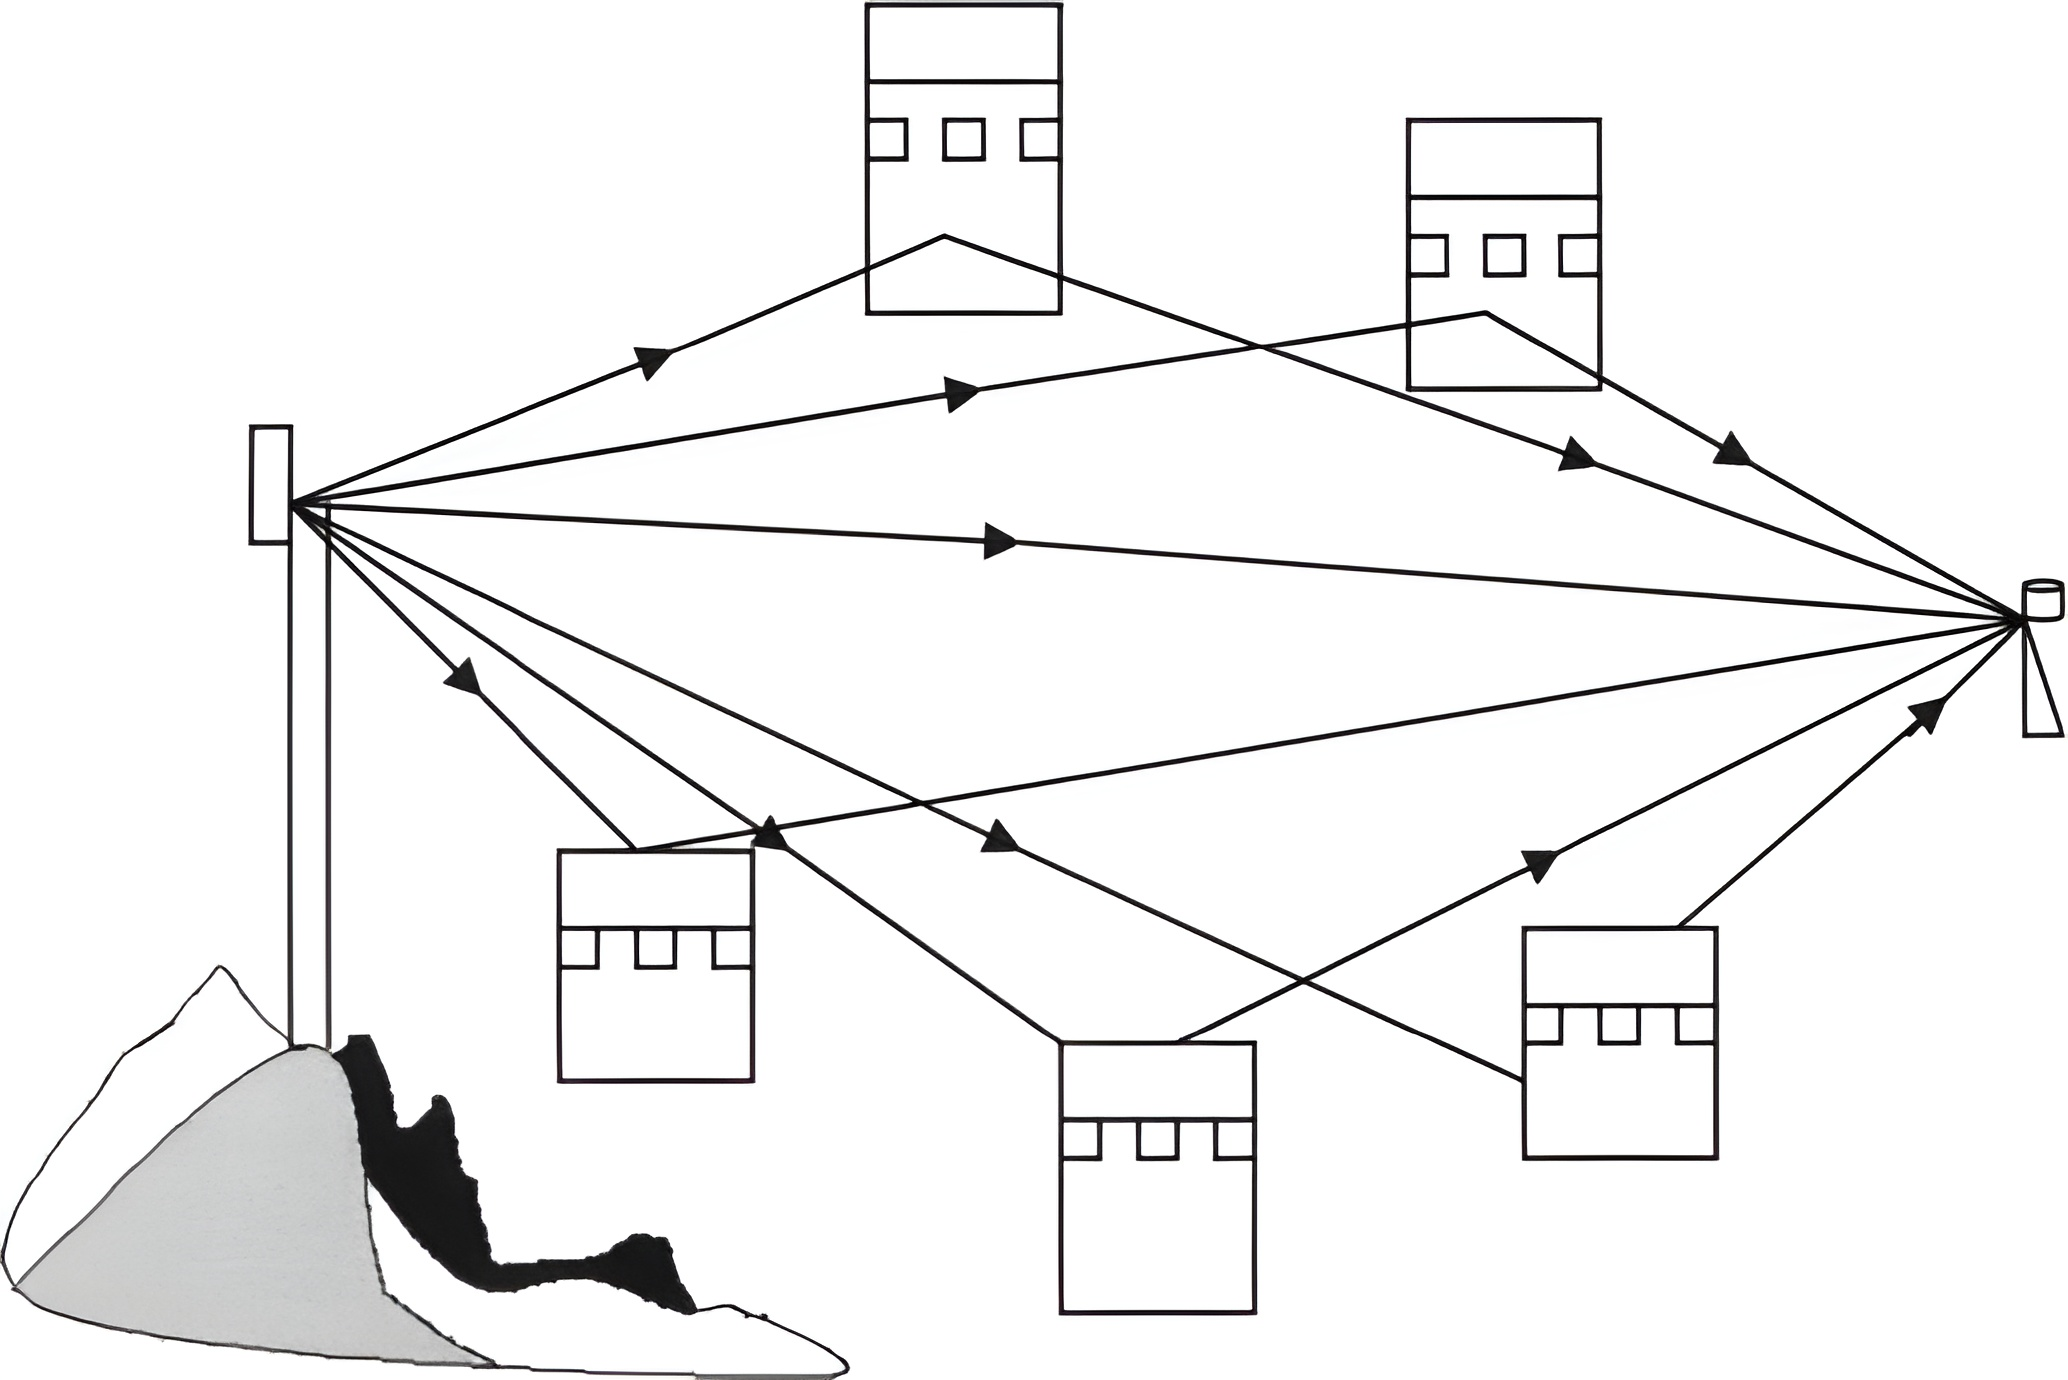
\includegraphics[width=0.92\textwidth]{Figures/multipath_propagation.png}
    \caption{\bfseries Illustration of multipath propagation phenomena}
    \label{fig:multipath}
\end{figure}

Orthogonal Frequency Division Multiplexing (OFDM) was developed to combat
frequency-selective fading by dividing a high-rate data stream into many
low-rate parallel subcarriers. Since each subcarrier experiences a nearly
flat fading channel, equalization becomes significantly simpler compared
to conventional single-carrier systems.

The OFDM transmitted signal can be represented mathematically using the
Inverse Fast Fourier Transform (IFFT):

\begin{equation}
\label{eq:ofdm_signal}
x[n]=\frac{1}{N}\sum_{k=0}^{N-1}X_k e^{j\frac{2\pi kn}{N}}
\end{equation}

where:
\begin{itemize}
    \item $X_k$ denotes the modulated data symbol on the $k$-th subcarrier,
    \item $N$ is the FFT size,
    \item $x[n]$ is the time-domain OFDM signal.
\end{itemize}

The orthogonality between subcarriers allows efficient spectrum usage
while avoiding inter-carrier interference (ICI).

\vspace{0.3cm}

\begin{figure}[H]
    \centering
    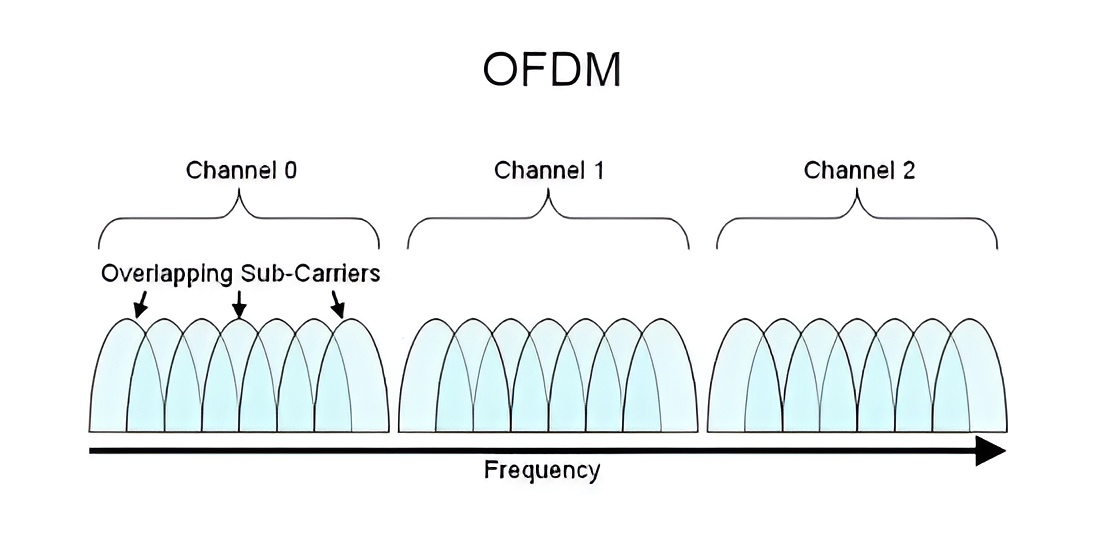
\includegraphics[width=0.9\textwidth]{Figures/ofdm_subcarriers.png}
    \caption{\bfseries Orthogonal overlapping subcarriers in OFDM systems}
    \label{fig:ofdm_subcarriers}
\end{figure}

Although OFDM provides excellent spectral efficiency and robustness
against multipath fading, one major drawback is its high
Peak-to-Average Power Ratio (PAPR). Since an OFDM signal is formed by the
superposition of many independently modulated subcarriers, constructive
interference occasionally produces extremely large signal peaks.

The PAPR of a transmitted signal is defined as:

\begin{equation}
\label{eq:papr}
\mathrm{PAPR}=
\frac{\max |x(t)|^2}
{E\{|x(t)|^2\}}
\end{equation}

where:
\begin{itemize}
    \item $\max |x(t)|^2$ is the peak instantaneous power,
    \item $E\{|x(t)|^2\}$ denotes the average signal power.
\end{itemize}

High PAPR reduces the efficiency of power amplifiers because the amplifier
must operate with large power back-off to avoid nonlinear distortion and
signal clipping.

%\vspace{0.3cm}

%\begin{figure}[H]
%    \centering
%    \includegraphics[width=0.92\textwidth]{Figures/papr_example.png}
%    \caption{\bfseries Example of large signal peaks in OFDM waveforms}
%    \label{fig:papr_example}
%\end{figure}

To address this limitation, Single-Carrier Frequency Division Multiple
Access (SC-FDMA) was introduced as an uplink transmission technique for
Long Term Evolution (LTE) systems. SC-FDMA combines the advantages of
single-carrier transmission and OFDM by inserting a Discrete Fourier
Transform (DFT) spreading operation before OFDM modulation.

The DFT spreading operation is expressed as:

\begin{equation}
\label{eq:dft_spreading}
X[m]=\sum_{n=0}^{M-1}d[n]e^{-j\frac{2\pi mn}{M}}
\end{equation}

where:
\begin{itemize}
    \item $d[n]$ represents the input modulation symbols,
    \item $X[m]$ denotes the spread frequency-domain symbols,
    \item $M$ is the number of occupied subcarriers.
\end{itemize}

By spreading information symbols across multiple subcarriers, SC-FDMA
produces a signal with lower envelope fluctuation and lower PAPR compared
to conventional OFDM.

\vspace{0.3cm}

\begin{figure}[H]
    \centering
    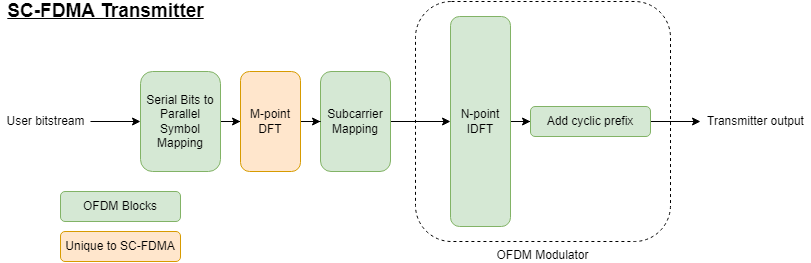
\includegraphics[width=0.95\textwidth]{Figures/ofdm_vs_scfdma_transmitter_blockdiagram.png}
    \caption{\bfseries Comparison between OFDM and SC-FDMA transmitter structures}
    \label{fig:ofdm_scfdma_compare}
\end{figure}

For this reason, SC-FDMA was selected for LTE uplink transmission, where
mobile devices require high power efficiency and long battery lifetime.

%============================================================%
\subsection{Problem Statement}

Despite its many advantages, OFDM suffers from high PAPR, which creates
practical implementation challenges in wireless transmitters. Large signal
peaks reduce power amplifier efficiency and increase nonlinear distortion,
leading to spectral regrowth and degraded transmission quality.

Although SC-FDMA was developed to reduce the PAPR problem, its
performance characteristics differ from OFDM due to the DFT spreading
operation. Therefore, a detailed comparison between OFDM and SC-FDMA is
necessary to understand the tradeoff between transmission performance,
power efficiency, and implementation complexity.

Furthermore, multipath fading channels introduce frequency-selective
distortion that affects both systems differently. Equalization techniques
must therefore be applied at the receiver to recover transmitted data and
maintain reliable communication.

%============================================================%
\subsection{Objectives}

The main objectives of this report are summarized as follows:

\begin{itemize}
    \item To study the operating principles of OFDM and SC-FDMA systems.
    
    \item To analyze the impact of multipath fading channels on system
    performance.
    
    \item To implement OFDM and SC-FDMA transmission systems using MATLAB.
    
    \item To evaluate system performance using Bit Error Rate (BER)
    analysis under different Signal-to-Noise Ratio (SNR) conditions.
    
    \item To compare the Peak-to-Average Power Ratio (PAPR) performance
    using Complementary Cumulative Distribution Function (CCDF)
    analysis.
    
    \item To discuss the engineering tradeoff between transmission
    reliability and power efficiency.
\end{itemize}

%============================================================%
\subsection{Scope of the Study}

This report focuses on the simulation and analysis of OFDM and localized
SC-FDMA systems under multipath Rayleigh fading channels. The systems are
implemented using 16-QAM modulation with identical FFT size, cyclic prefix
length, active subcarrier allocation, and transmission bandwidth for fair
comparison.

The receiver employs Zero Forcing (ZF) equalization to compensate for
channel distortion in the frequency domain.

The study mainly focuses on:
\begin{itemize}
    \item BER performance comparison,
    \item PAPR analysis,
    \item multipath fading effects,
    \item frequency-domain equalization.
\end{itemize}

The following topics are outside the scope of this report:
\begin{itemize}
    \item channel coding,
    \item MIMO transmission,
    \item adaptive modulation,
    \item interleaved SC-FDMA mapping,
    \item advanced equalization techniques such as MMSE.
\end{itemize}

%============================================================%
\subsection{Report Structure}

This report is organized into the following chapters:

\begin{itemize}
    \item Chapter 1 introduces the background, motivation, objectives,
    and scope of the study.
    
    \item Chapter 2 presents the theoretical foundations of OFDM,
    SC-FDMA, multipath fading, PAPR, and equalization techniques.
    
    \item Chapter 3 describes the simulation methodology, system
    parameters, channel model, and MATLAB implementation.
    
    \item Chapter 4 presents simulation results and discusses BER and
    PAPR performance comparisons between OFDM and SC-FDMA.
    
    \item Chapter 5 summarizes the main conclusions and proposes future
    research directions.
\end{itemize}

\newpage
\clearpage